\documentclass[13.5pt,aspecratio=169, xcolor=dvipsnames]{beamer}
\usepackage{graphicx} % Required for inserting images
\usepackage{subcaption}
\usepackage{amsfonts}
\usepackage{amsmath}
\usepackage{amssymb}
\usepackage{physics}
\usepackage{bm}
\usepackage{physics}
\usepackage{booktabs}
\usepackage{setspace}
\usepackage{xcolor}
\usepackage{wrapfig,lipsum}
\usetheme{Madrid}
\useinnertheme{circles}

\DeclareMathOperator*{\argmax}{arg\,max}
\DeclareMathOperator*{\argmin}{arg\,min}
\graphicspath{{Images/}{./}} 
\usetheme{Copenhagen}
\definecolor{UBCblue}{rgb}{0.04706, 0.13725, 0.26667} 
\usecolortheme[named=UBCblue]{structure}
%\usecolortheme{beaver}
\title{Spot The Differences Between Two Images}
\author[CS231]{\textit{Le Gia Khang \\ Le Duy Khang \\ Nguyen Hoang Tan }\\ \bigskip \textbf{CS231: Introduction to Computer Vision}}
\date{\today}
\definecolor{mylightgreencolor}{RGB}{144, 238, 144}
\definecolor{mylightredcolor}{RGB}{255, 204, 203}
\setbeamertemplate{navigation symbols}{}
\setbeamertemplate{headline}{}
\setbeamercolor{huge text}{fg=white}
\setbeamertemplate{footline}{
    \leavevmode%
    \hbox{%
        \begin{beamercolorbox}[wd=.2\paperwidth,ht=2.25ex,dp=1ex,center]{author in head/foot}%
            \usebeamerfont{author in head/foot}\insertshortauthor
        \end{beamercolorbox}%
        \begin{beamercolorbox}[wd=.7\paperwidth,ht=2.25ex,dp=1ex,center]{title in head/foot}%
            \usebeamerfont{title in head/foot}\insertshorttitle
        \end{beamercolorbox}%
        \begin{beamercolorbox}[wd=.1\paperwidth,ht=2.25ex,dp=1ex,right]{date in head/foot}%
            \insertframenumber{} / \inserttotalframenumber\hspace*{2ex} 
        \end{beamercolorbox}%
    }%
    \vskip0pt%
}

\begin{document}
\maketitle

% \begin{frame}
% 	\frametitle{Table of Contents} % Slide title, remove this command for no title
% 	\tableofcontents[subsectionstyle=hide]
% \end{frame}
%-------------------------------------------------------------------%


\begin{frame}
    \doublespacing
        \frametitle{Presentation Overview} % Slide title, remove this command for no title
        
        \tableofcontents % Output the table of contents (all sections on one slide)
        %\tableofcontents[pausesections] % Output the table of contents (break sections up across separate slides)
\end{frame}
    
    %----------------------------------------------------------------------------------------
    %	PRESENTATION BODY SLIDES
    %----------------------------------------------------------------------------------------
    
    \section{Problem Statement} % Sections are added in order to organize your presentation into discrete blocks, all sections and subsections are automatically output to the table of contents as an overview of the talk but NOT output in the presentation as separate slides
    %------------------------------------------------
    \begin{frame}
        \doublespacing
            \frametitle{Presentation Overview} % Slide title, remove this command for no title
            
            \tableofcontents[currentsection] % Output the table of contents (all sections on one slide)
            %\tableofcontents[pausesections] % Output the table of contents (break sections up across separate slides)
    \end{frame}

%-------------------------------------------------------------------%

\subsection{Why it Matters}
\begin{frame}
    \onehalfspacing
        \frametitle{Why it Matters}
        
        \begin{minipage}{0.55\textwidth}
            \begin{minipage}{0.9\textwidth}
            \begin{block}{Applications}
                Detecting changes is a natural computer
                vision task:
                \begin{itemize}
                    \item The “spot-the-difference” game
                    \item Facility monitoring
                    \item Medical imaging
                    \item Satellite surveillance
                    \item Counterfeit detection
                \end{itemize}
                ... and many more.
            \end{block}
        \end{minipage}
        \end{minipage}
        \begin{minipage}{0.4\textwidth}
            \begin{figure}[h]
            \includegraphics[scale=0.55]{Medical_Imaging.jpg}
            \begin{center}
            \hspace{1em} Comparison of two MRI \\ \hspace{1em} scans over 10-year period. 
            \end{center}
            \end{figure}
        \end{minipage}
    \end{frame}
    
    %--------------------------------------------------
    \subsection{Input and Output Analysis}

    \begin{frame}
    \onehalfspacing
        \frametitle{Input and Output Analysis}
            \begin{block}{\begin{center}Input\end{center}}
                \vspace{1em}
                \begin{center}Pair of images need to compare \hphantom{with bounding boxes to indicate
                    areas of distinction
                    }\end{center}
                
                \begin{figure}
                    \centering
                    \includegraphics[scale=0.3]{Example/07_full.jpg}
                \end{figure}
            \end{block}
    \end{frame}
    
    
    %------------------------------------------------
    \begin{frame}
        \onehalfspacing
            \frametitle{Input and Output Analysis}
                \begin{block}{\begin{center}Output\end{center}}
                    \vspace{1em}
                    \begin{center}The provided images are marked with bounding boxes \\ to indicate areas of distinction\end{center}
                    
                    \begin{figure}
                        \centering
                        \includegraphics[scale=0.3]{Example/7_res_full.png}
                    \end{figure}
                \end{block}
        \end{frame}
    
    %------------------------------------------------
    
    \subsection{Examples}

    \begin{frame}
    \onehalfspacing
        \frametitle{Examples: Input}
        \hspace{1em}
        \includegraphics[scale=0.5]{Example/Fishing_boy.png}
    \end{frame}
    %------------------------------------------------

    \begin{frame}
        \onehalfspacing
            \frametitle{Examples: Input}
            \begin{figure}[h]
            \centering
            \includegraphics[scale=0.5]{Example/Camera_1.png}
            \end{figure}
        \end{frame}
        %------------------------------------------------

        \begin{frame}
            \onehalfspacing
                \frametitle{Examples: Input}
                \begin{figure}[h]
                \centering
                \includegraphics[scale=0.5]{Example/Example_1.png}
                \end{figure}
            \end{frame}
            %------------------------------------------------
    

            \begin{frame}
            \onehalfspacing
                \frametitle{Examples: Output}
                \hspace{1em}
                \includegraphics[scale=0.5]{Example/Fishing_boy_bb.png}
            \end{frame}
            %------------------------------------------------
        
            \begin{frame}
                \onehalfspacing
                    \frametitle{Examples: Output}
                    \begin{figure}[h]
                    \centering
                    \includegraphics[scale=0.4]{Example/Camera_1_bb.png}
                    \end{figure}
                \end{frame}
                %------------------------------------------------
        
                \begin{frame}
                    \onehalfspacing
                        \frametitle{Examples: Output}
                        \begin{figure}[h]
                        \centering
                        \includegraphics[scale=0.5]{Example/Example_1_bb.png}
                        \end{figure}
                    \end{frame}
                    %------------------------------------------------
            

    
\section{Methodology} % Sections are added in order to organize your presentation into discrete blocks, all sections and subsections are automatically output to the table of contents as an overview of the talk but NOT output in the presentation as separate slides
\begin{frame}
	\frametitle{Presentation Overview} % Slide title, remove this command for no title
	\tableofcontents[currentsection]
\end{frame}

%------------------------------------------------
% {
% \begin{frame}
% 	\frametitle{Methods for POS Tagging and NER}
%     \setbeamertemplate{footline}{boo \insertframenumber}
%     \begin{minipage}{0.5\textwidth}  % Adjust the width as needed
%         {
%         \setbeamercolor{block body}{bg=mylightgreencolor} % Block body color
%         \begin{block}{} % Block without title
%             HMM – Hidden Markov chains
%         \end{block}
%         }
%         \begin{block}{} % Block without title
%             CRF – Conditional Random Fields
%         \end{block}
        
%     \end{minipage}\hspace{10pt}
%     \begin{minipage}{0.45\textwidth}  % Adjust the width as needed
%             \centering
%             \includegraphics[scale=0.3]{POS-Tagging.jpg}
%     \end{minipage}
	
    
% \end{frame}
% }

%------------------------------------------------
\subsection{Pixel-Wise Comparison}
\subsection{Siamese Network}
\begin{frame}
    \onehalfspacing
        \frametitle{Siamese Network}
        Proposed in the article "The Change You Want To See" accepted at the IEEE/CVF Winter Conference on Application of Computer Vision 2023.
        \bigskip
        \begin{figure}
            \begin{subfigure}{0.5\textwidth}
              \centering
              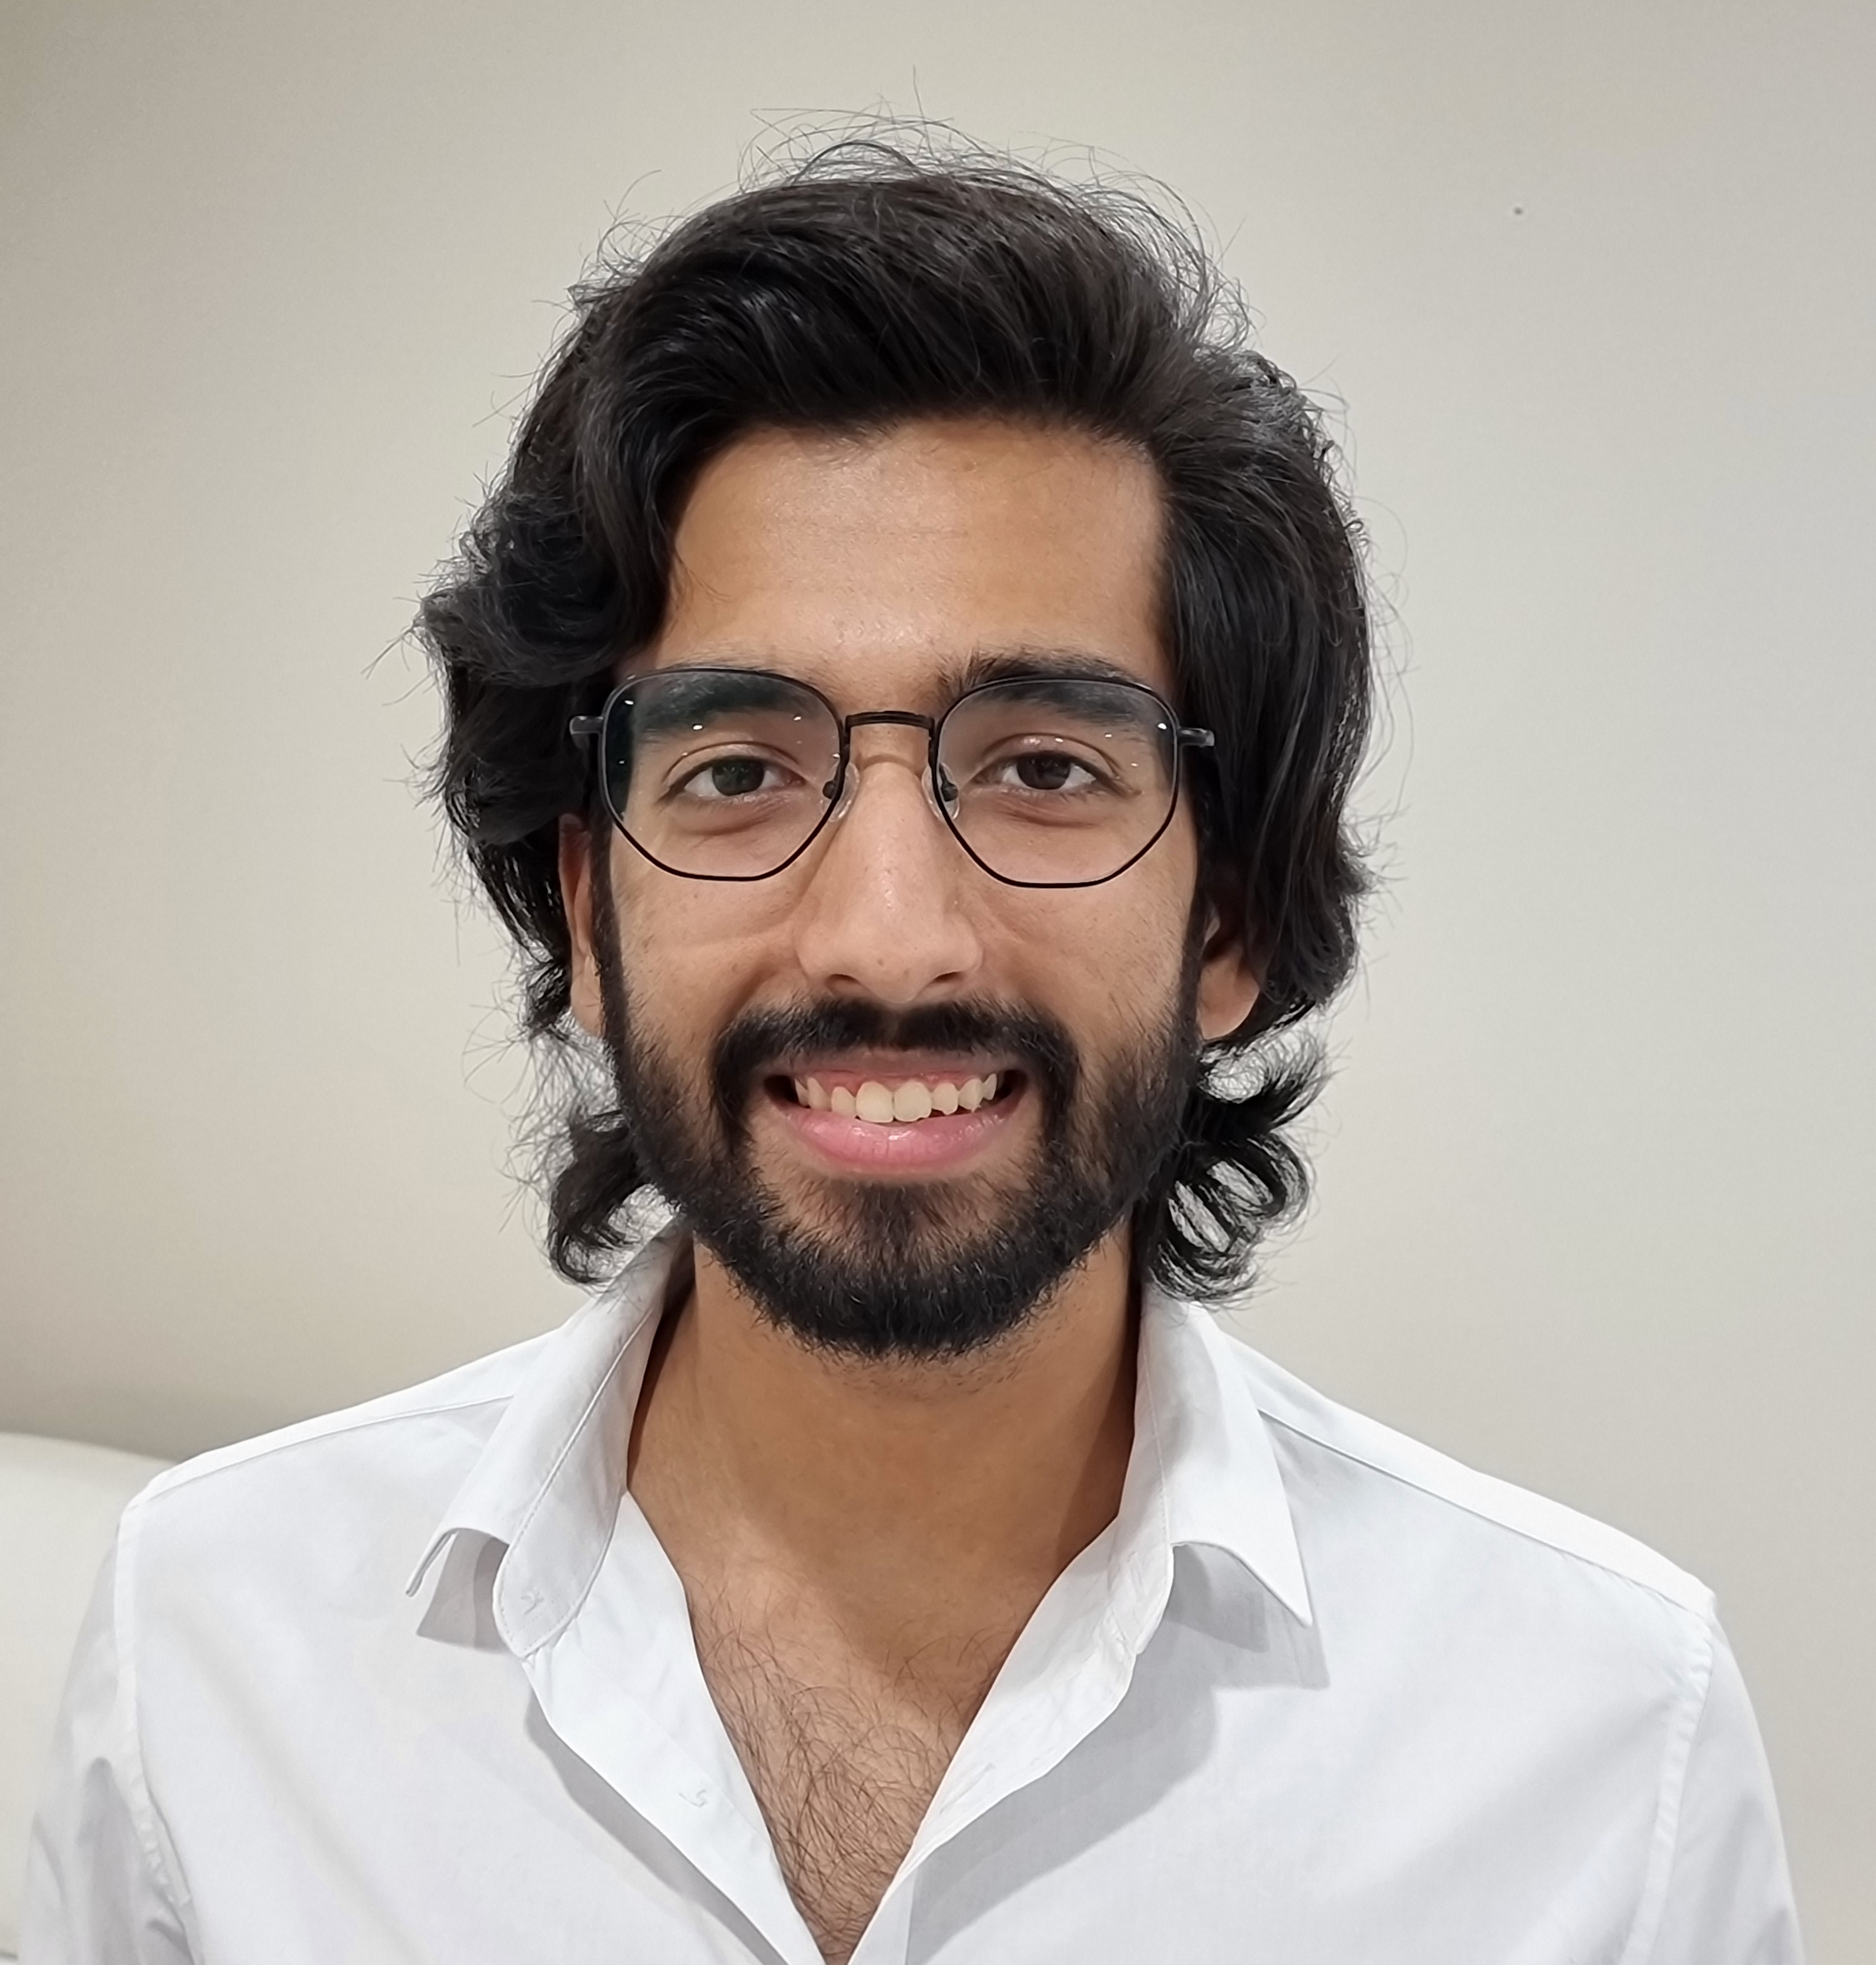
\includegraphics[width=0.7\linewidth]{Regav.png}
              \captionsetup{labelformat=empty}
              \caption{Ragav Sachdeva}
              \label{fig:subfig1}
            \end{subfigure}%
            \begin{subfigure}{0.5\textwidth}
              \centering
              \includegraphics[width=0.7\linewidth]{Zisserman.jpg}
              \captionsetup{labelformat=empty}
              \caption{Andrew Zisserman}
              \label{fig:subfig2}
            \end{subfigure}
            \captionsetup{labelformat=empty}
            \caption{Visual Geometry Group at the University of Oxford}
            \label{fig:overall}
        \end{figure}
      
\end{frame}
    
%------------------------------------------------

\begin{frame}
    \onehalfspacing
        \frametitle{Siamese Network: Overview}
        \begin{itemize}
            \item Enable “object-level” change prediction and simplify counting the number of changes between two images.
            \item Use an architecture that operates on two images with
            geometric (scale, rotation,..) and photometric changes.
            \item Designed to be
            class-agnostic, it can detect changes irrespective of
            the object classes involved. 
        \end{itemize}
        
        \begin{figure}
            \centering
            \includegraphics[scale=0.5]{Siamese_network_1.png}
        \end{figure}
        
\end{frame}

%------------------------------------------------


\begin{frame}
    \onehalfspacing
        \frametitle{Model Architecture Overview}
        \begin{figure}
            \centering
            \includegraphics[width=\linewidth]{Siamese_network_architecture.png}
            \caption{\textbf{Architecture}: Utilizing a dual-image encoder, feature maps $(f^s_1, f^s_2)$ are generated. A co-attention module aligns and conditions these maps $(g^s_1, g^s_2)$. Subsequently, a U-Net decoder processes the original and conditioned maps to yield final feature maps $(h_1, h_2)$. The bounding box detector head employs $h_1$ and $h_2$ to generate bounding boxes for images $I_1$ and $I_2$, respectively}
        \end{figure}
        
\end{frame}

%------------------------------------------------



\begin{frame}
\onehalfspacing
	\frametitle{Siamese Network: Overview}
    \begin{block}{Siamese Network}
        A type of neural network architecture designed for tasks involving similarity or distance measurement between input pairs. 
        \begin{itemize}
            \item Consists of two identical subnetworks (or twins) that share the same set of weights and parameters.
            \item The name originates from Chang (left) and Eng Bunker (right).
        \end{itemize}
    \end{block}

    \begin{figure}
        \centering
        \includegraphics[scale=0.3]{Siamese_Twin.jpg}
    \end{figure}
\end{frame}

%------------------------------------------------
\begin{frame}
    \onehalfspacing
        \frametitle{Siamese Network: Architecture}
        
       \begin{itemize}
            \item Consists of two identical subnetworks.
            \item Extract feature vectors from both networks using a common set of convolutional and fully connected layers.
            \item Feature vectors from both networks are compared using a loss function $L$.
       \end{itemize}
       \begin{figure}
            \centering
            \includegraphics[scale=0.5]{Siamese_architecture.png}
       \end{figure}
        
\end{frame}
%------------------------------------------------
\begin{frame}
    \onehalfspacing
        \frametitle{U-Net Encoder-Decoder Network}
        U-Net is a type of convolutional neural network (CNN) architecture commonly used for image segmentation tasks.
        \begin{minipage}{0.55\textwidth}
            \begin{minipage}{0.95\textwidth}
            \begin{block}{Consists of an encoder-decoder structure:}
                \begin{itemize}
                    \item \textbf{Encoder:} capturing features from the input image. 
                    \item \textbf{Decoder:} upsampling and producing a segmented output.
                \end{itemize}
            \end{block}
        \end{minipage}
        \end{minipage}
        \begin{minipage}{0.35\textwidth}
            \begin{figure}[h]
                \centering
                \hspace{10em}
                \includegraphics[scale=0.4]{U_net.png}
            \end{figure}
        \end{minipage}

        \vspace{2em}
        The authors employed \textbf{ResNet50} as the CNN for the encoder.
\end{frame}
%------------------------------------------------

\begin{frame}
    \onehalfspacing
        \frametitle{A UNet encoder-decoder with CoAM}
        
        \begin{block}{CoAM Attention Module}
            We wish to concatenate features from both images in order to condition the model on both input images.
            \begin{itemize}
                \item However, for a given spatial location, the
                relevant feature in the other image may not be at the same spatial location.
            \end{itemize}
            As a result, we use an
            attention mechanism to model long range dependencies.
        \end{block}
        \begin{figure}[h]
            \centering
            \includegraphics[width=\linewidth]{CoAM_model.png}
            \caption{Correspondences obtained with the CoAM model, which is augmented with an attention mechanism. }
        \end{figure}
\end{frame}
%------------------------------------------------

\begin{frame}
\onehalfspacing
	\frametitle{A UNet encoder-decoder with CoAM}
    \begin{figure}[h]
        \centering
        \includegraphics[width=\linewidth]{Co_Attention_Module.png}
    \end{figure}
\end{frame}
%------------------------------------------------

\begin{frame}
    \onehalfspacing
        \frametitle{Use Siamese network to detect changes}
            \begin{figure}[h]
                \centering
                \includegraphics[scale=0.4]{Siamese_network_architecture.png}
            \end{figure}
        
            \begin{itemize}
                \item First obtaining a set of dense feature
                descriptors for each image using a CNN-based (ResNet50) encoder.
                \item These feature are then conditioned on
                each other using a co-attention mechanism that implicitly
                supplies the correspondences.

            \end{itemize}
    \end{frame}
    %------------------------------------------------


\begin{frame}
    \onehalfspacing
        \frametitle{Use Siamese network to detect changes}
            \begin{figure}[h]
                \centering
                \includegraphics[scale=0.4]{Siamese_network_architecture.png}
            \end{figure}
        
            \begin{itemize}
                \item Next, feature are passed through a decoder to obtain high
                resolution conditioned image descriptors which are used
                by a bounding box detection head to localise the changes.
            \end{itemize}
    \end{frame}
    %------------------------------------------------


\begin{frame}
    \onehalfspacing
        \frametitle{Siamese Network: Dataset}
        For this method, we make use of a state-of-the-art image inpainting method, \textbf{LaMa}, to make the objects \textit{disappear}. 
        \begin{figure}[h]
            \centering
            \includegraphics[width=\linewidth]{Lama.png}
        \end{figure}
    \end{frame}
%------------------------------------------------
\begin{frame}
    \onehalfspacing
        \frametitle{Siamese Network: Dataset}
       
            \begin{itemize}
                \item We also apply random affine transformations to the images along with colour jittering or add random text to “background” images.
                \item Datasets: COCO-Inpainted, Synthtext-Change, VIRAT-STD, Kubric-Change.
                
            \end{itemize}

            \begin{figure}[h]
                \centering
                \includegraphics[width=\linewidth]{Siamese_dataset.png}
            \end{figure}

    \end{frame}

%------------------------------------------------


\onehalfspacing
\begin{frame} % Use [allowframebreaks] to allow automatic splitting across slides if the content is too long
	\frametitle{Reference}
	
	\begin{thebibliography}{99} % Beamer does not support BibTeX so references must be inserted manually as below, you may need to use multiple columns and/or reduce the font size further if you have many references
		\footnotesize % Reduce the font size in the bibliography
		
		\bibitem[Stanford]{p1}
			The Change You Want To See
			\newblock Ragav Sachdeva and Andrew Zisserman

        \bibitem[Stanford]{p1}
            Understanding SSIM
			\newblock Jim Nilsson and Tomas Akenine-Möller
			
	\end{thebibliography}
\end{frame}



%	CLOSING SLIDE
%----------------------------------------------------------------------------------------

\begin{frame} % The optional argument 'plain' hides the headline and footline
	\begin{center}
		{\Huge Thanks for listening!}
		
		\bigskip\bigskip % Vertical whitespace
		
		{\LARGE Q\&A section}
	\end{center}
\end{frame}
%------------------------------------------------


\end{document}
